\newpage
\section{Problem 1: Time Series Match Prediction Based on Long Short-Term Memory Network}
% \lipsum[1-4] \cite{1}
\subsection{Data Preprocessing}
Within the dataset provided by MCM, there exists a comprehensive collection of 46 attributes pertaining to tennis matches, comprising 38 numerical attributes and 8 categorical ones.

The following is the data processing method we adopted:
\begin{itemize}[label=$\bullet$]
  \item We numerically encoded 4 of the categorical attributes: winner\_shot\_type, serve\_width, serve\_depth, and return\_depth.
  \item Given the convention in tennis scoring where "AD" signifies an advantage, which is challenging to quantify, we use the fields "p1\_score" and "p2\_score" as equivalent numerical representations of the scores.
  \item For handling missing values in numerical data and ensuring the continuity of the data, we use the Lagrange interpolation method. For a given set of \(n+1\) data points, the Lagrange interpolation polynomial is given by:
  \begin{equation}
       P(x) = \sum_{i=0}^{n} f(x_i) \cdot L_i(x) 
  \end{equation}

where \(L_i(x)\) represents the Lagrange basis function.


   \item There are still 42 fields remaining, except for the four fields match\_id, player1, player2, and elapsed\_time. Due to the large number of fields, we conducted dimensionality reduction on the data.
   \item Because of  the non-uniformity of data dimensions, it is not possible to observe the degree and trend of changes in various attributes simultaneously. Therefore, we performed Min-Max Normalization processing.
  \begin{equation}
       x_{\text{normalized}} = \frac{x - \text{min}(x)}{\text{max}(x) - \text{min}(x)} 
  \end{equation}
\end{itemize}








Additionally, before dimensionality reduction, we need to calculate the correlation between each field, and we choose to calculate the Spearman rank correlation coefficient between each field to measure the monotonic relationship between two variables, which not only takes into account the linear relationship between the variables, but also takes into account their rank relationship, which is more robust to data that do not satisfy the assumption of normal distribution. The formula for the Spearman's rank correlation coefficient is as follows:

\begin{equation}
\rho=\frac{\sum_{i=1}^n\left(R(x_i)-\overline{R(x)}\right )\cdot \left(R(y_i)-\overline{R(y)}\right)}{\sqrt{\left(\sum_{i=1}^n\left(R(x_i)-\overline{R(x)}\right)^2\right)\cdot\left(\sum_{i=1}^n\left(R(y_i)-\overline{R(y)}\right)^2\right)}}\end{equation}

In this equation, $\rho$ deotes the Spearman rank correlation coefficient, n is the number of data points, $R(x_i)$ and $R(y_i)$ denote the ranks of variables $x$ and $y$, respectively, and $\overline{R(x)}$ and $\overline{R(y)}$ denote the means of the ranks of $x$ and $y$, respectively.

The Spearman’s rank correlation coefficient analysis results between any two fields take values between -1 and 1. The closer the value is to 1 or -1, the stronger the correlation between the two fields. Conversely, the closer the value is to 0, the weaker the correlation between the two fields. A correlation heatmap between some fields, calculated based on Spearman’s rank correlation coefficient, is shown in Figure \ref{fig:correlation_heatmap }.



\begin{figure}[h]
    \centering
    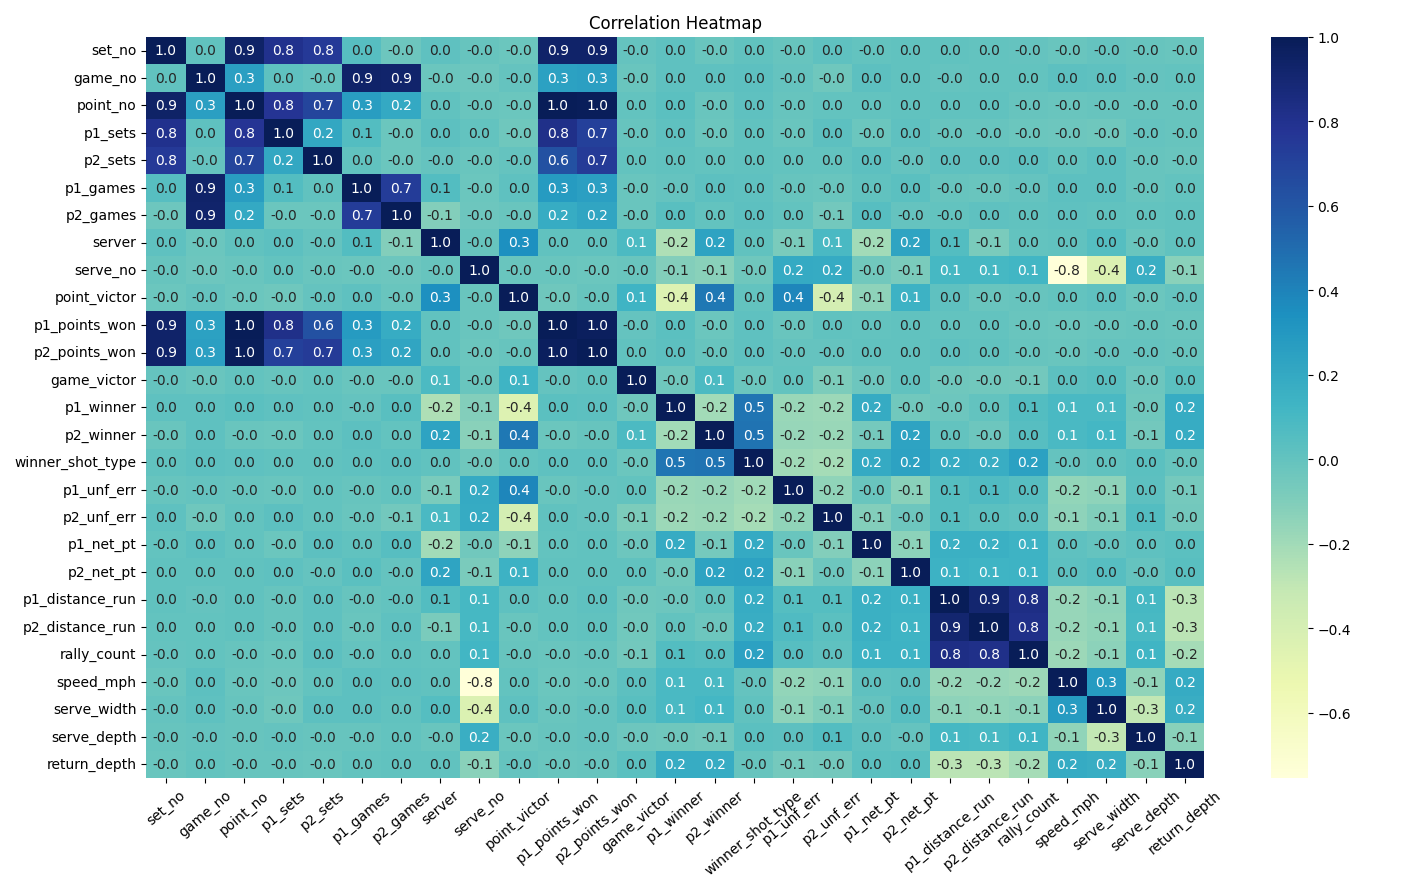
\includegraphics[width=1.05\textwidth]{figure/correlation heatmap.png}
     % \vspace{-0.3cm}
    \caption{Correlation Heatmap Based on Spearman Correlation Analysis
    \textnormal{}}
    \label{fig:correlation_heatmap }
    % \vspace{-0.5cm}
\end{figure}

According to the correlation heatmap, the correlation coefficients between the distance run by the two players in the match ("p1\_distance\_run", "p2\_distance\_run") and the number of strokes in the match ("rally\_count") are $\geq 0.8$, which indicates that there is a strong correlation between them. It can be understood that the more the number of hits in the game, the longer the distance run in the game, so we only keep the number of hits in the game ("rally\_count") field, and delete the distance run by the two players in the game ("p1\_distance\_run", "p2\_distance\_run"), so as to achieve the effect of the data dimensionality reduction. Based on this kind of correlation analysis, we did dimensionality reduction on the data, extracted some fields that are more independent from each other, and finally extracted 27 fields for subsequent model training.




\subsection{Model Structure}\label{sec:model_structure}
On a real field of play, the game situation has the following insight into the impact of the game on the player: the closer the point is to the current game, the greater the impact on the player.\cite{insight} Therefore, to simulate this effect, we modeled a long and short-term memory network based model to capture the flow of points occurring while the game is in progress.


Long Short-Term Memory (LSTM) is a special kind of Recurrent Neural Network (RNN), widely used in the field of Natural Language Processing.The core idea of LSTM is its so-called "Cell state" and its interaction with three gate controllers: Input Gate, Forget Gate, Output Gate. During the training process, the network learns the parameters of these three gate controllers dynamically. Through the collaboration of the three gates, the LSTM can selectively remember or forget information, and therefore can efficiently process sequences of different lengths. Figure \ref{fig:lstm_struction} shows the exact structure of the LSTM model we built.

\begin{figure}[htbp]
    \centering
    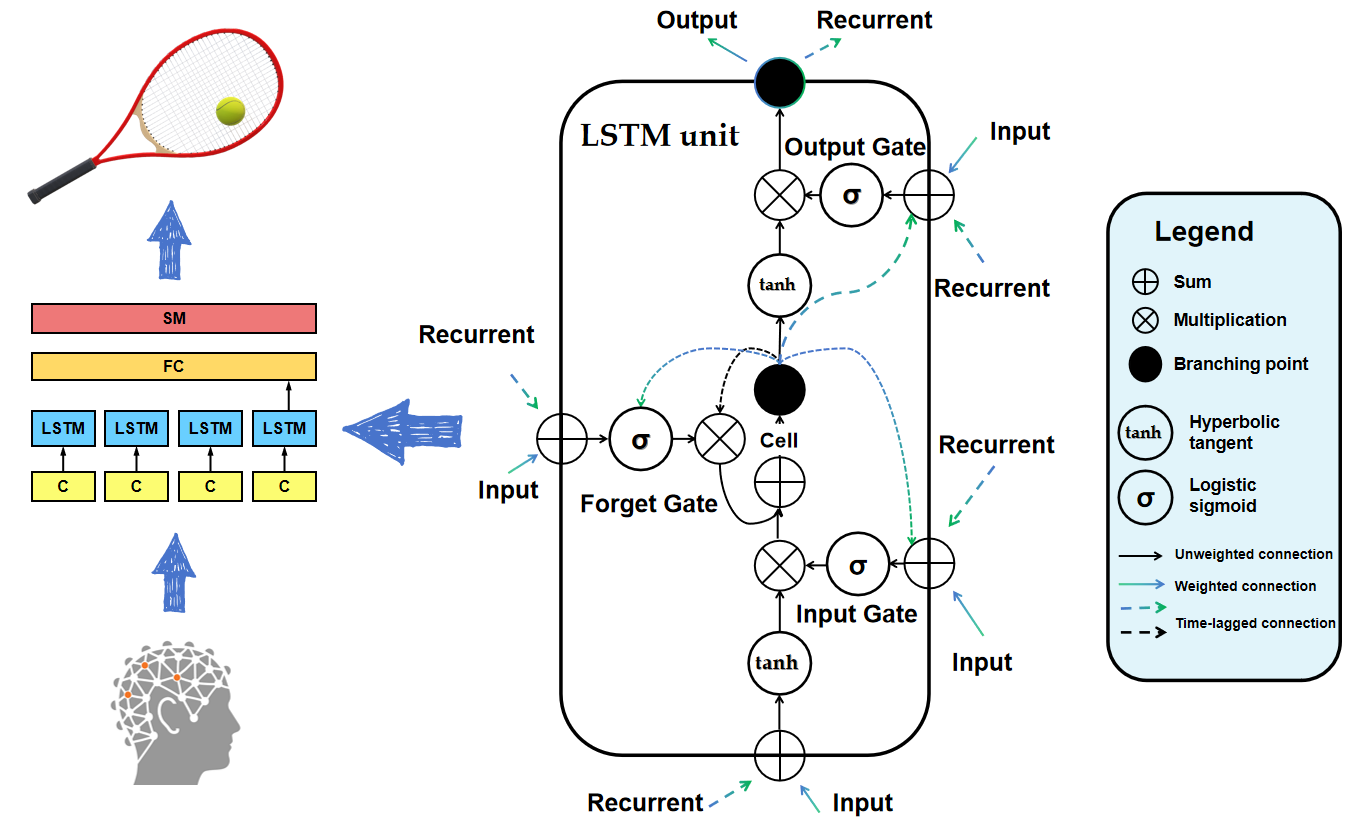
\includegraphics[width=0.9\textwidth]{figure/lstm_structure.png}
    % \vspace{-0.3cm}
    \caption{The Structure Diagram of LSTM
    \textnormal{}}
    \label{fig:lstm_struction}
    % \vspace{-0.5cm}
\end{figure}

We employ LSTM to simulate players' behavior during a match. In this simulation, the Cell state in LSTM represents the player's current match status, the Input Gate simulates the player's reception of current changes on the field, the Forget Gate simulates the player's forgetting of previous match conditions, and the Output Gate simulates the actions taken by the player based on the current match status. Additionally, we construct a sequence of dimensionally reduced point data from a match, which serves as the input to the model and is denoted as $x_t$ . Specifically:


\begin{itemize}[label=\textbf{\normalsize$\bullet$}]
    \item Input Gate determine what new information will be added to the unit state, similar to how an player adjusts his or her tactics and techniques in a game based on the current round and the opponent's strategy. We denote the input gate as $I_t$. The expression of $I_t$ is:
    % 这是输入门的变量取值
    \begin{equation}I_{t}=\sigma(x_{t}\cdot k_{1}+h_{t-1}\cdot k_{2}+b_{1})\end{equation}

    \item Forget Gate determines which information in the unit state should be discarded, similar to how an player ignores or forgets the favorable and unfavorable factors of previous rounds in a game in order to focus on the current challenge. In the current match, information that is further away from the present is more likely to be discarded by the oblivion gate, and their impact on the current situation gradually diminishes. This is similar to the human brain's forgetting curve. We denote the forget gate as $F_t$. The expression of $F_t$ is:
    % 这是遗忘门的变量取值
    \begin{equation}F_{t}=\sigma(x_{t}\cdot k_{3}+h_{t-1}\cdot k_{4}+b_{2})\end{equation}
    \item Output Gate determine which parts of the unit's state will be used to generate the current output, similar to how an player decides their next move based on the current round and previous experience. We denote the output gate as $O_t$. The expression of $O_t$ is:
    % 这是输出门的变量取值
    \begin{equation}O_{t}=\sigma(x_{t}\cdot k_{5}+h_{t-1}\cdot k_{6}+b_{3})\end{equation}
    \end{itemize}
    
During the training process, the Cell state is updated based on the Input Gate and Forget Gate, after which the Output Gate forms the output based on the value of the Cell state.
% \begin{figure}[htbp]
%     \centering
%     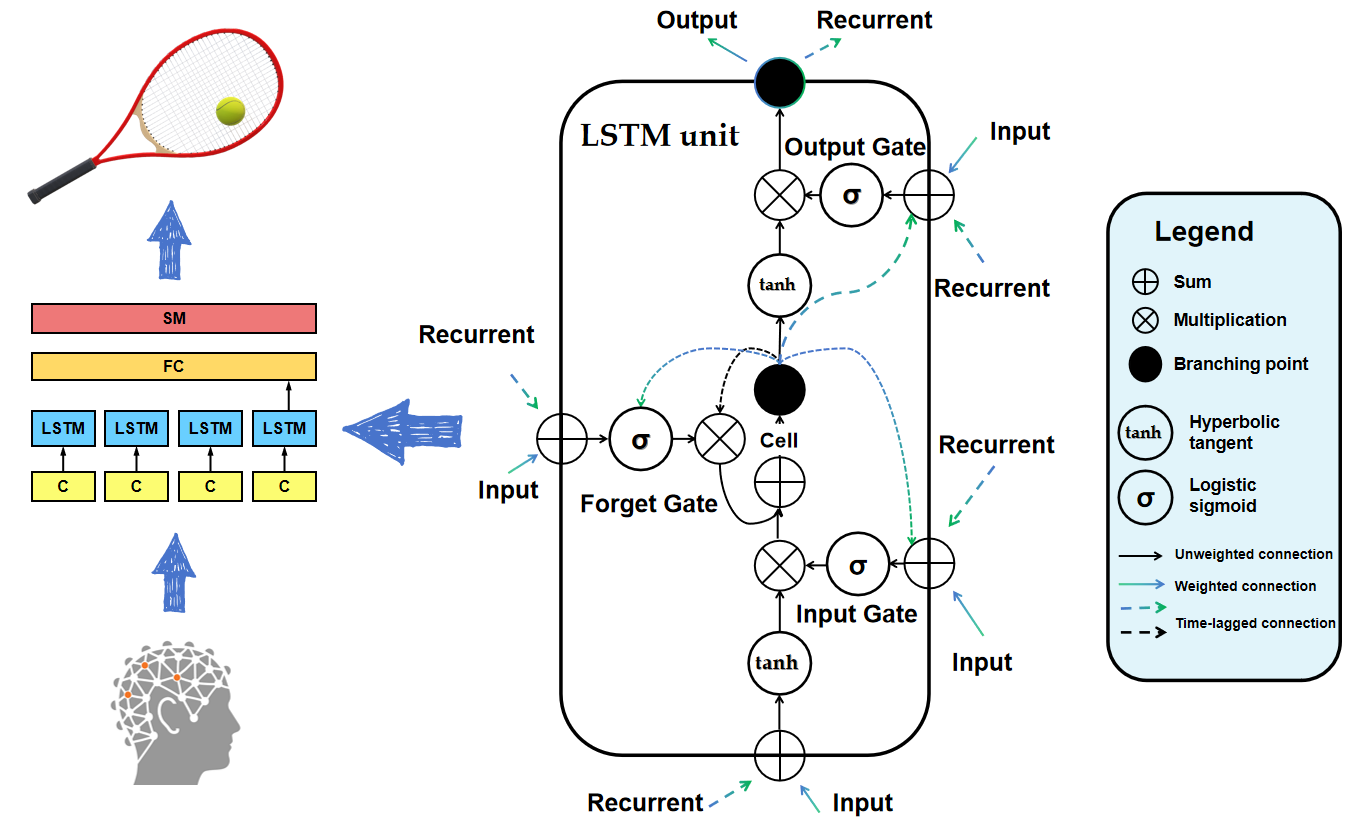
\includegraphics[width=0.9\textwidth]{figure/lstm_structure.png}
%     % \vspace{-0.3cm}
%     \caption{The structure diagram of LSTM
%     \textnormal{}}
%     \label{fig:lstm_struction}
%     % \vspace{-0.5cm}
% \end{figure}

\subsection{Training and Predicting Results}
We utilize the dataset provided by MCM, allocating \(90\%\) of the data for model training and the remaining \(10\%\) for testing. After iterating through 1000 training epochs, the model's loss function values are presented in Figure \ref{fig:lstm_loss}. The results indicate that our model achieves an accuracy rate of \(94.52\%\) on unseen data, demonstrating its robust generalization capabilities to accurately predict players' scores in real match scenarios.

% \vspace*{-10pt}
\begin{figure}[htbp]
  \centering
  \subfigure[Training Loss]{%
    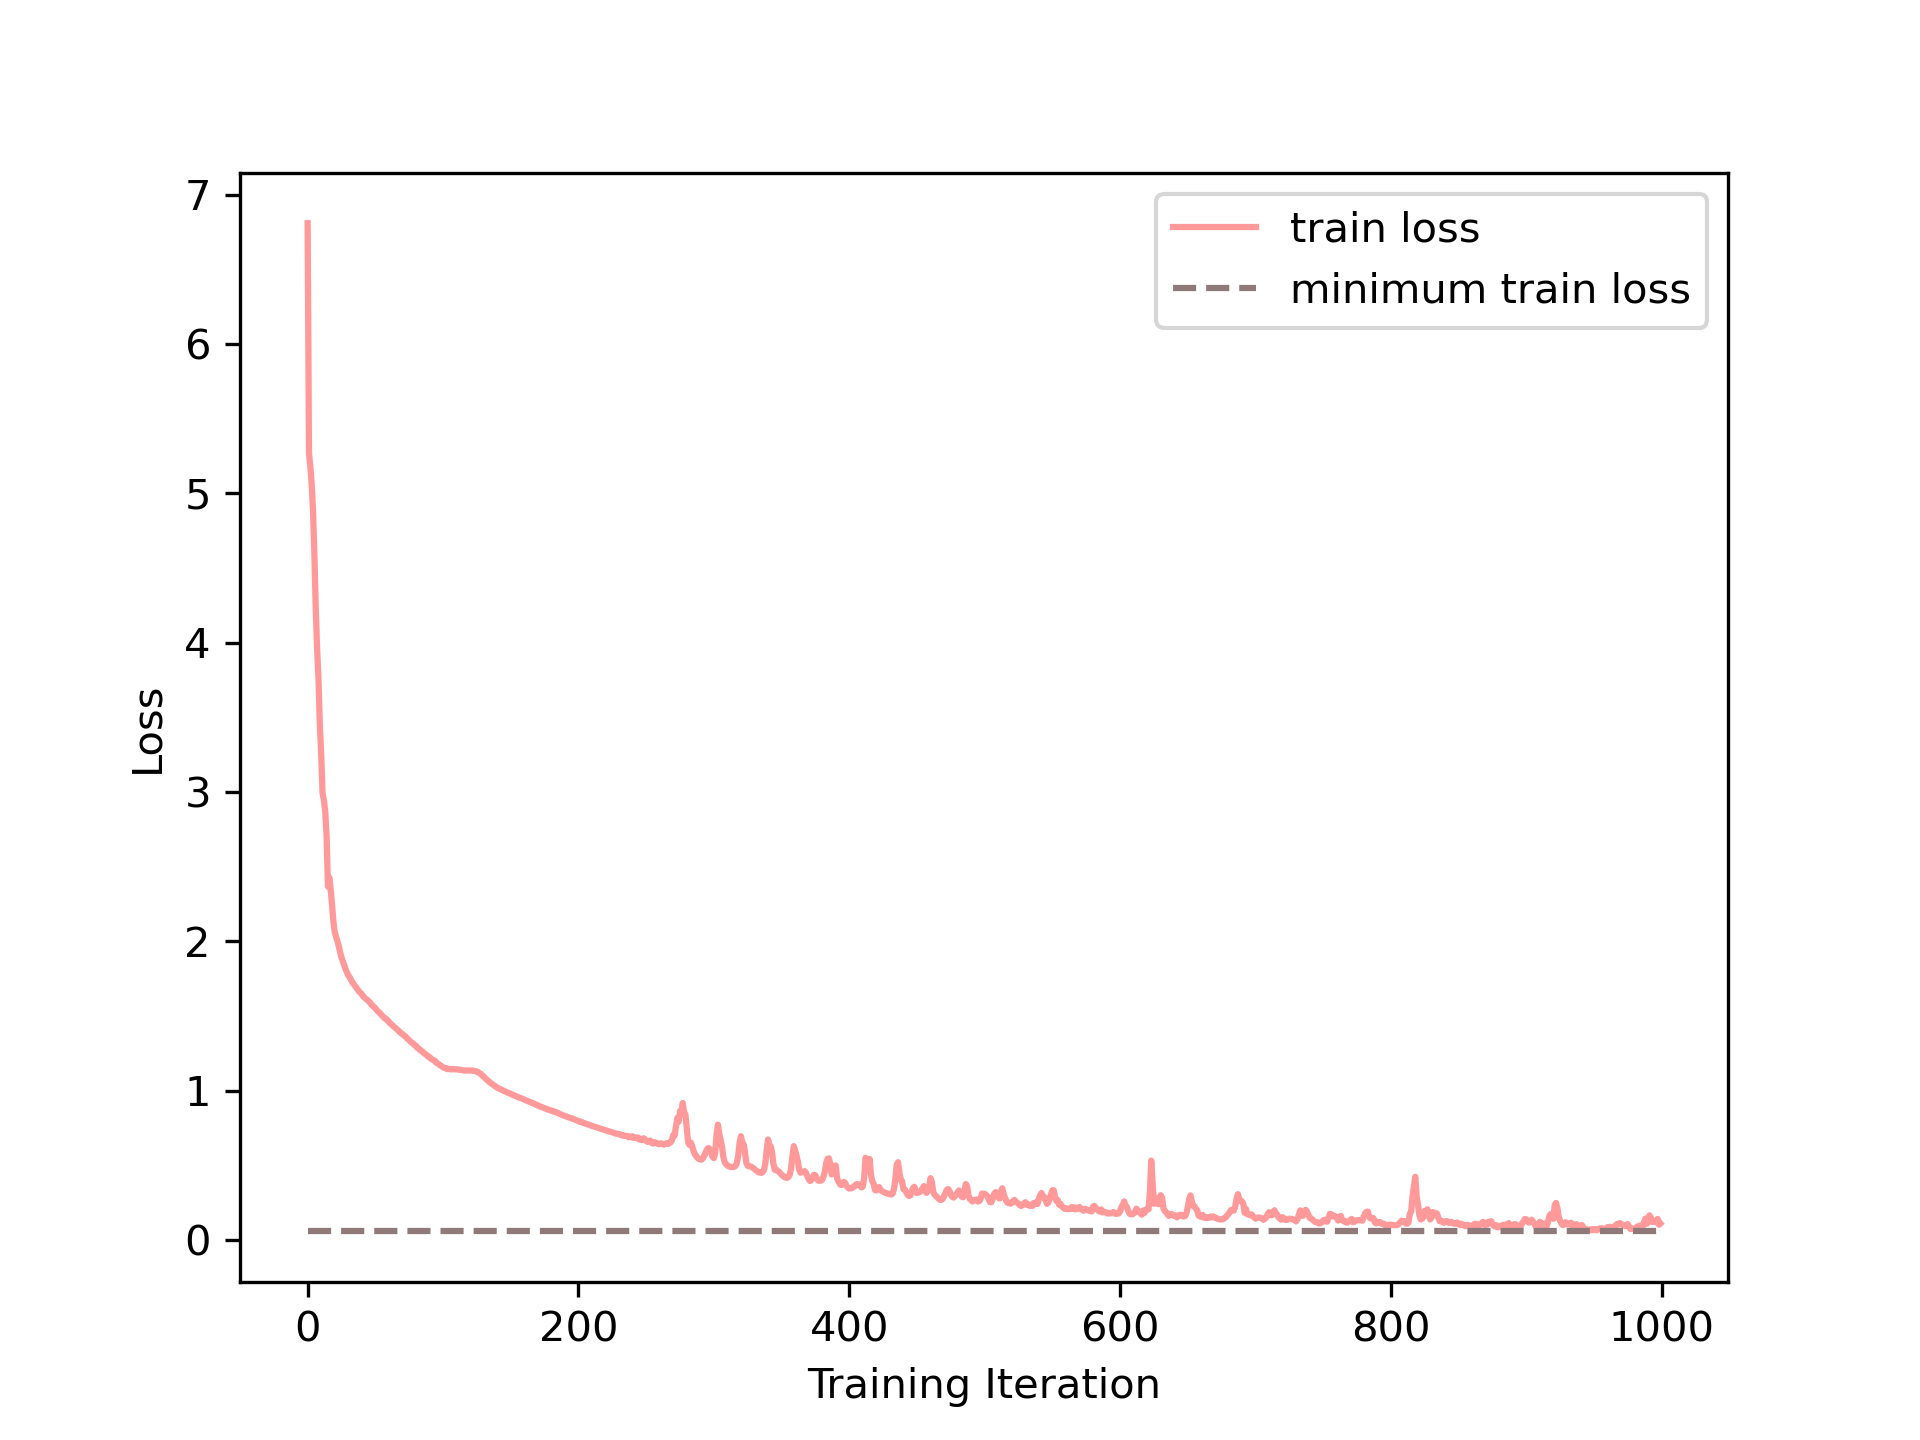
\includegraphics[width=0.48\textwidth]{figure/loss_curve_lstm_train.png}
    \label{fig:train_loss}
  }
  \subfigure[Testing Loss]{%
    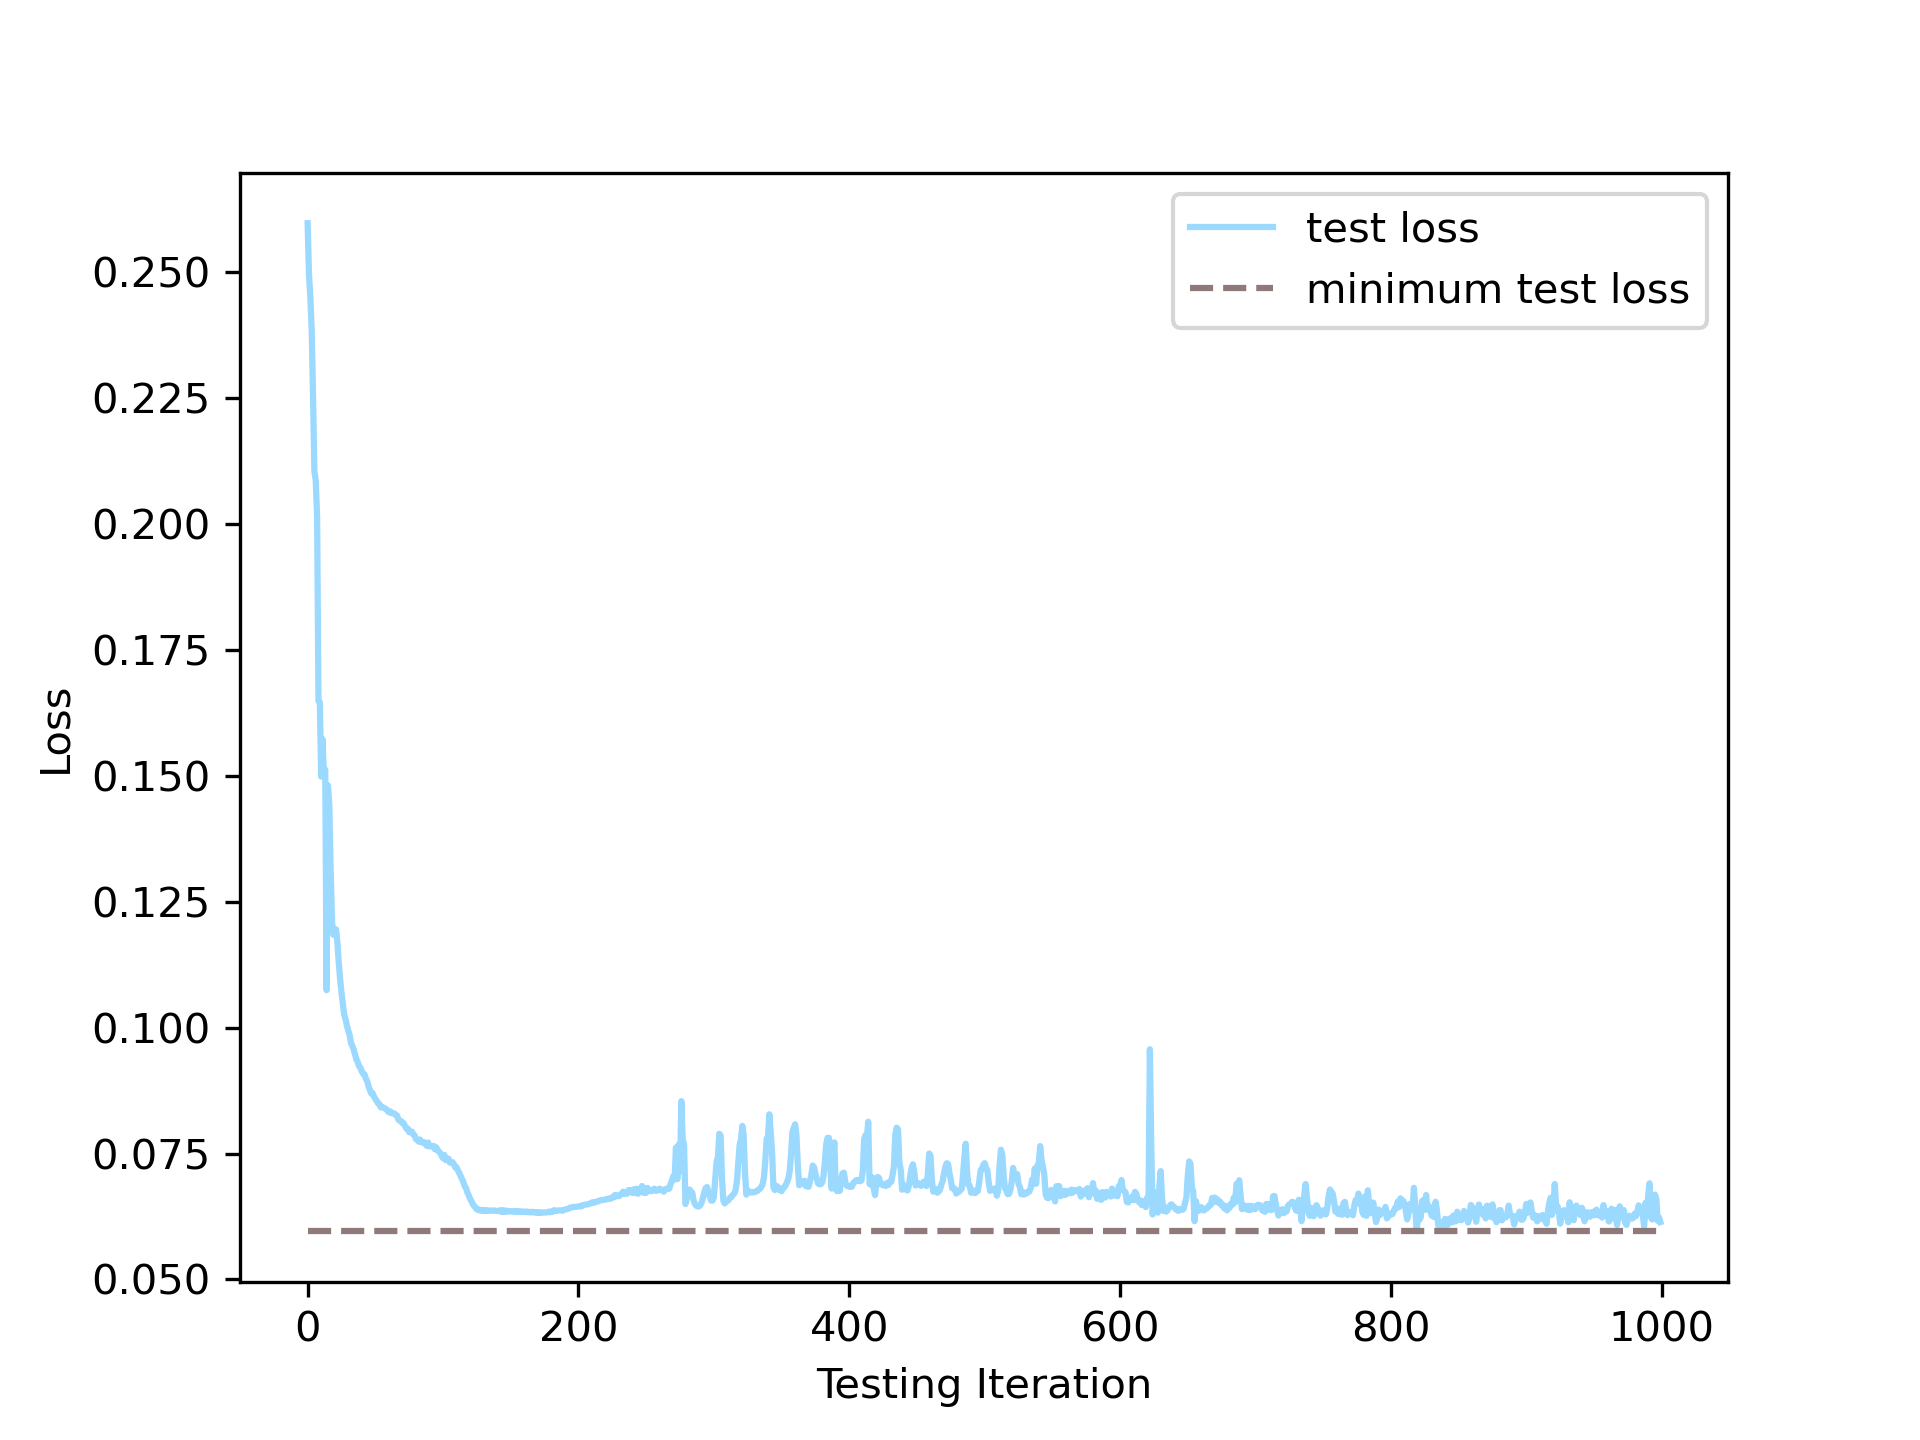
\includegraphics[width=0.48\textwidth]{figure/loss_curve_lstm_test.png}
    \label{fig:test_loss}
  }
  \caption{The Loss Curve for MM-LSTM}
  \label{fig:lstm_loss}
\end{figure}

Based on this, we visualized the match process between Carlos Alcaraz and Novak Djokovic (whose data was not used for training) as shown in Figure \ref{fig:match_visual}. The X-axis represents the flow of the match, with the blue section representing Carlos Alcaraz and the green section representing Novak Djokovic. We used the area of the bar chart to represent the performance score of the player at the current moment, with both players’ performance scores ranging between 0 and 1, summing up to 1. The player with the higher performance score at each moment is predicted to be the winner of the game.

\begin{figure}[htbp]
    \centering
    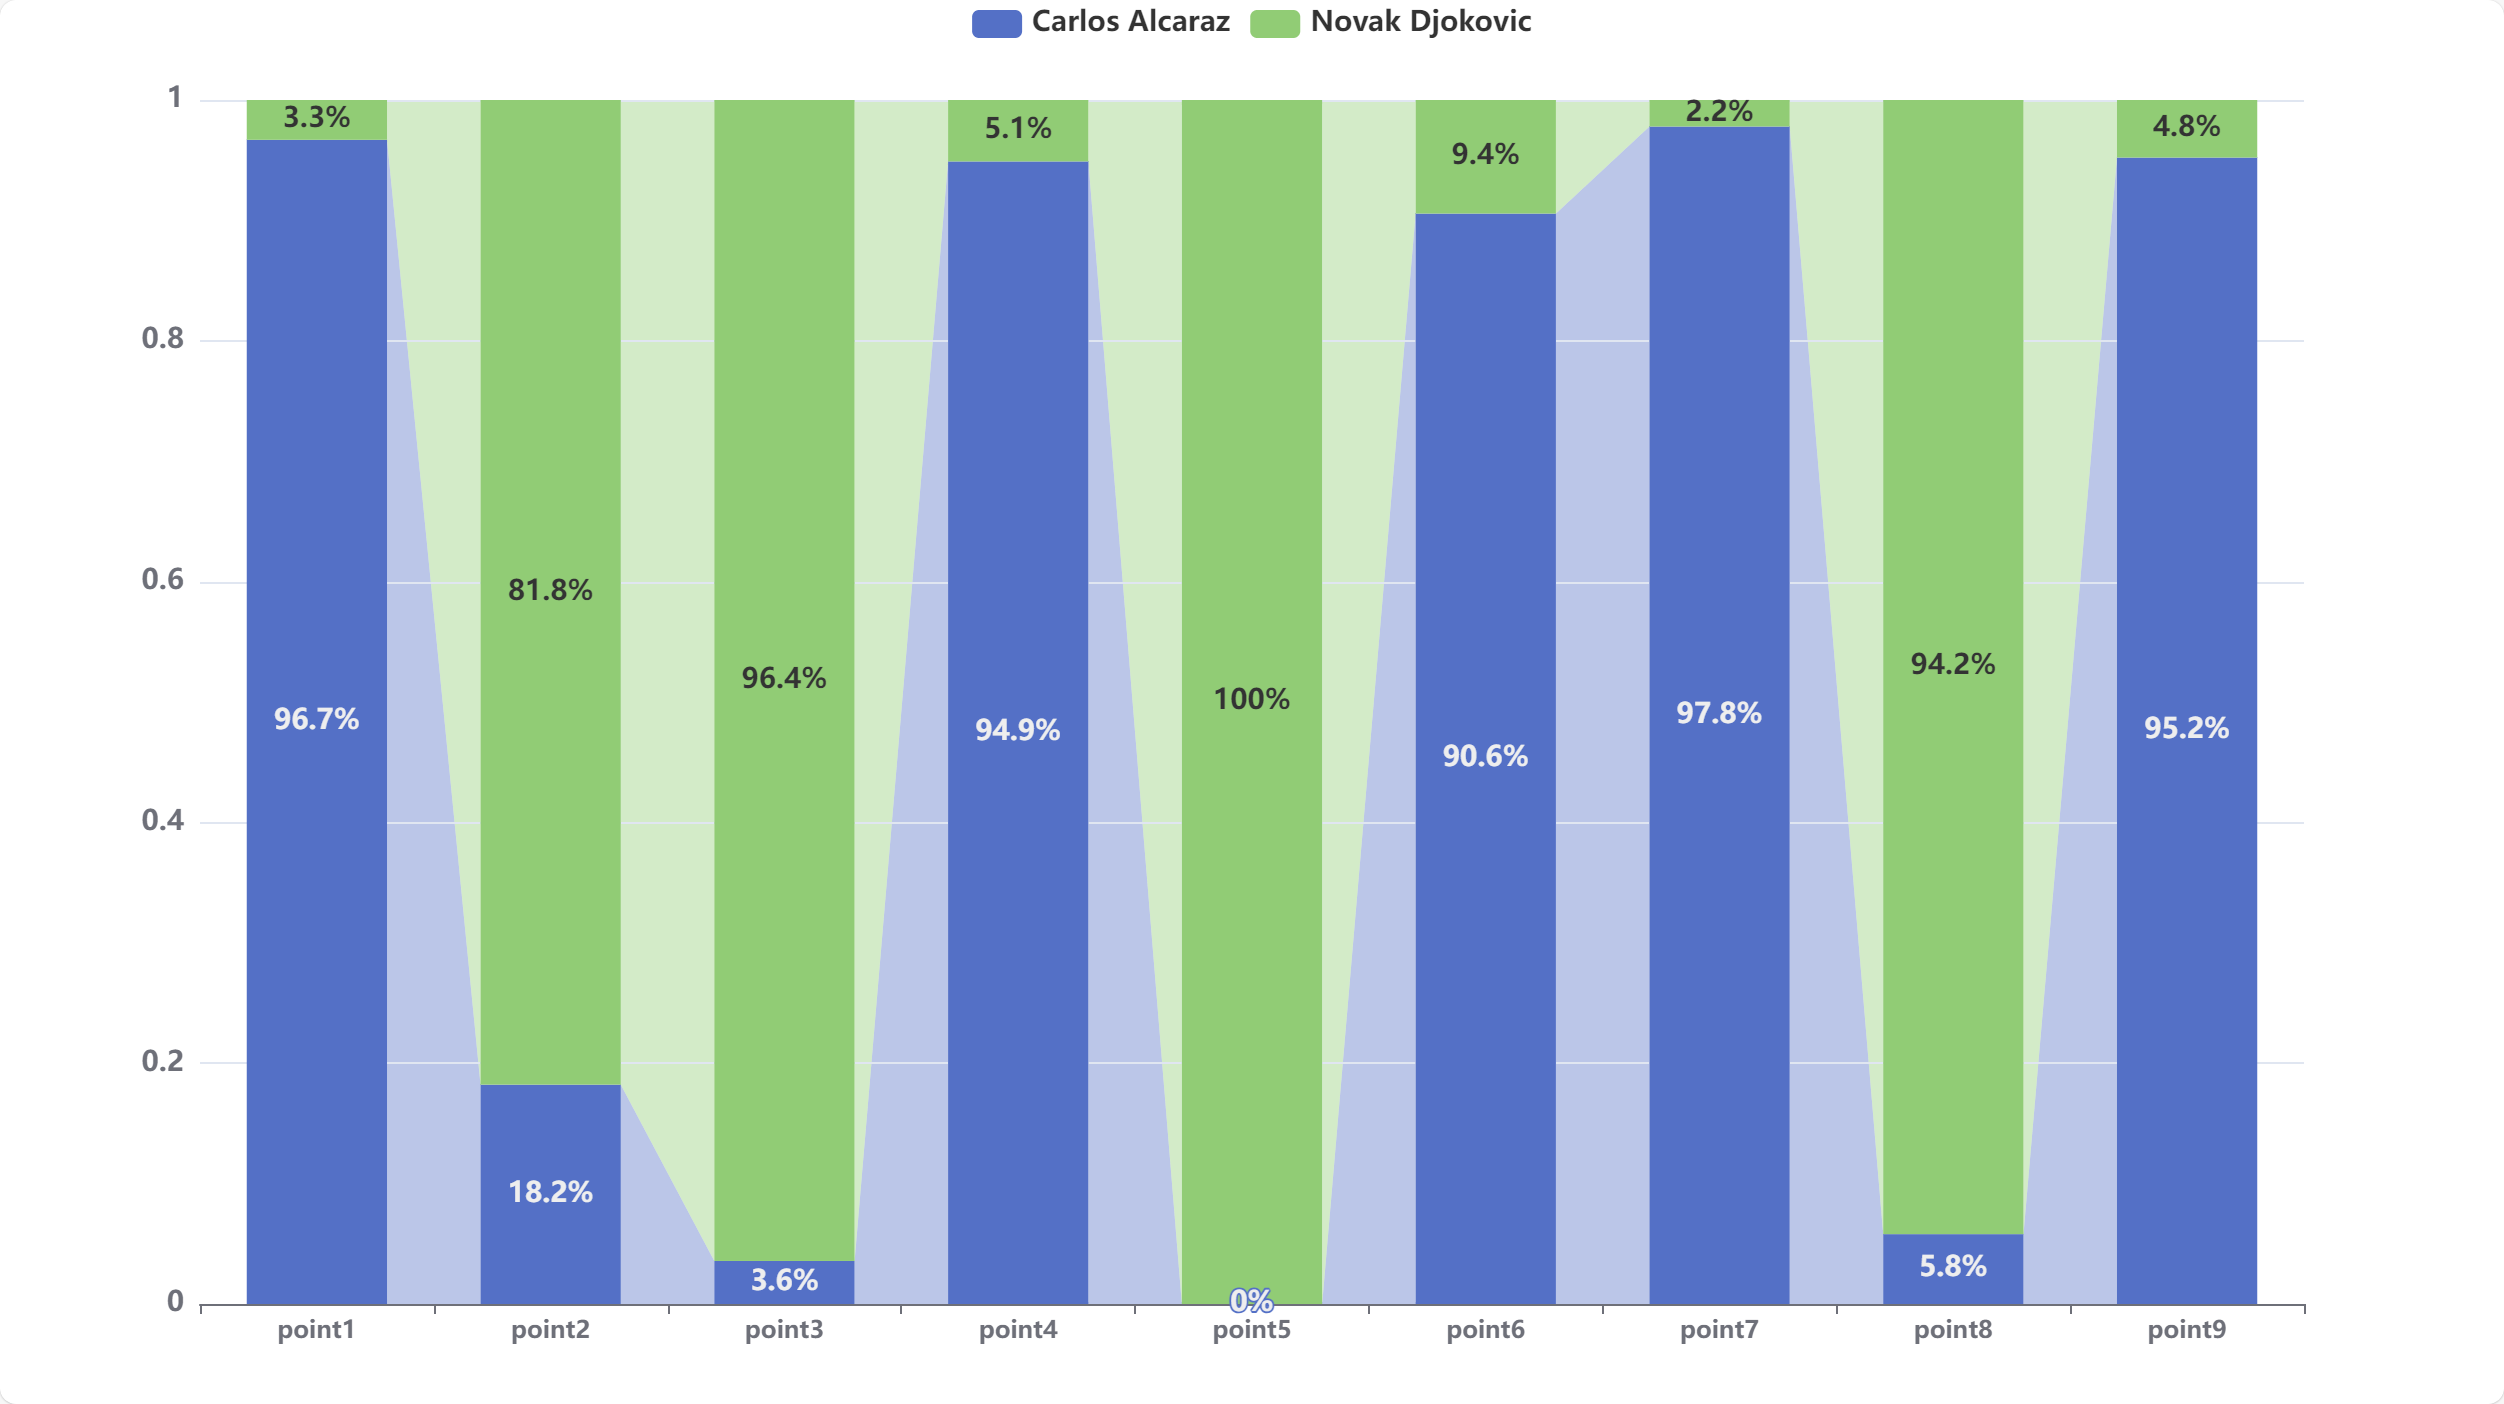
\includegraphics[width=0.95\textwidth]{figure/match_visual.png}
    % \vspace{-0.3cm}
    \caption{Match Flow Visualization: Carlos Alcaraz vs. Novak Djokovic
    \textnormal{}}
    \label{fig:match_visual}
    % \vspace{-0.5cm}
\end{figure}

% \subsection{Momentum-based LSTM Model Representation}
% To illustrate the correlation between our LSTM model and momentum, we simplify the modeled LSTM model into a well-formed momentum model based on the following equations.

% % The traditional momentum model is formulated as follows:
% % \begin{equation}
% % \begin{aligned}
% % p_* & =\sum p_i \\
% % & =\sum m_i v_i
% % \end{aligned}
% % \end{equation}

% Our LSTM model is formulated as follows, Our LSTM model is formulated as follows, where $I_t$, $F_t$, $O_t$, $C_t$ represent the input gate, forget gate, output gate, Cell state mentioned in Section 3.2, respectively:
% \begin{equation}
% \begin{gathered}
%     H_{t} = O_{t} \cdot \tanh(C_{t}) = O_{t} \cdot \tanh\left(F_{t} \cdot C_{t-1} + I_{t} \cdot \tilde C_{t}\right) \label{eq:lstm_base}
% \end{gathered}
% \end{equation}

% Based on the formula for input gate, forget gate, output gate mentioned in \ref{sec:model_structure}, we can expand the formula \ref{eq:lstm_base}:
% \begin{equation}
% \begin{gathered}
%     H_{t} = \sigma(x_{t} \cdot k_{5} + h_{t-1} \cdot k_{6} + b_{3}) \cdot \tanh\left(\sigma(x_{t} \cdot k_{3} + h_{t-1} \cdot k_{4} + b_{2}) \cdot C_{t-1} \right.\\
%     \quad \left. + \sigma(x_{t} \cdot k_{1} + h_{t-1} \cdot k_{2} + b_{1}) \cdot \tanh\left(x_{t} \cdot k_{7} + h_{t-1} \cdot k_{8} + b_{4}\right)\right)\label{eq:lstm_expand}
% \end{gathered}
% \end{equation}

% Simplify the formula \ref{eq:lstm_expand}:
% \begin{equation}
% f_{i}(x_{t}) = x_{t}\cdot k_{a_{i}(t)} + h_{t-1} \cdot k_{b_{i}(t)} + b_{c_{i}(t)}
% \end{equation}
% % 这是使用f代替后的表达式
% \begin{equation}H_{t} = \sigma\left( f_{1}(x_{t}) \right) \cdot \tanh\left( \sigma(f_{2}(x_{t})) \cdot C_{t-1} + \sigma(f_{3}(x_{t})) \cdot \tanh(f_{4}(x_{t})) \right)\label{eq:lstm_simply}
% \end{equation}

% We extract a part of the formula \ref{eq:lstm_simply}, denoted $P_n$:

% % 三个公式全都对齐
% % \begin{equation}\begin{aligned}P_n&=\sigma(f_2(x_t))\cdot C_{t-1}+\sigma(f_3(x_t))\cdot\tanh(f_4(x_t)))\\&=F_2(x_t)C_{t-1}+F_3(X_t)\cdot\tanh(f_4(X_t))\\&=A+B\cdot\tan h(F_4(x_t))\\&=A+\alpha(p)\\
% % A&=F_2(x_t)C_{t-1}+F_3(X_t)\\B&=F_3(x_t)\end{aligned}\end{equation}

% % 三个公式不对齐
% % \begin{equation}\begin{aligned}P_n&=\sigma(f_2(x_t))\cdot C_{t-1}+\sigma(f_3(x_t))\cdot\tanh(f_4(x_t)))\\&=F_2(x_t)C_{t-1}+F_3(X_t)\cdot\tanh(f_4(X_t))\\&=A+B\cdot\tan h(F_4(x_t))\\&=A+\alpha(p)\end{aligned}\end{equation}
% \begin{equation}\begin{aligned}P_n&=\sigma(f_2(x_t))\cdot C_{t-1}+\sigma(f_3(x_t))\cdot\tanh(f_4(x_t)))\\&=F_2(x_t)C_{t-1}+F_3(X_t)\cdot\tanh(f_4(X_t))\end{aligned}\end{equation}


% Then we simply Pn:
% % \begin{equation}A=F_2(x_t)C_{t-1}+F_3(X_t)\end{equation}
% % \begin{equation}B=F_3(x_t)\end{equation}
% % \begin{equation}P_n=A+B\cdot\tanh(F_4(x_t))=A+\alpha(p)\end{equation}
% % \begin{equation}\begin{aligned}P_n&=A+B\cdot\tanh(F_4(x_t))\\&=A+\alpha(p)\end{aligned}\end{equation}
% % \begin{equation}\begin{aligned}P_n&=\sigma(f_2(x_t))\cdot C_{t-1}+\sigma(f_3(x_t))\cdot\tanh(f_4(x_t)))\\&=F_2(x_t)C_{t-1}+F_3(X_t)\cdot\tanh(f_4(X_t))\\&=A+B\cdot\tanh(F_4(x_t))\\&=A+\alpha(p)\end{aligned}\end{equation}

% \begin{equation}
% \left\{
% \begin{aligned}
%     A &= F_2(x_t)C_{t-1}+F_3(X_t) \\
%     B &= F_3(x_t) \\
%     P_n &= A+B\cdot\tanh(F_4(x_t)) \\
%     &= A+\alpha(p)
% \end{aligned}
% \right.
% \end{equation}

% Thus, We can divide the formula in \ref{eq:lstm_simply} into two parts, $F_1$, $P_n$. $F_1$ denotes the function of the race at the current point in time, and Pn denotes the temporal part, which includes the content of the cell state in the LSTM, i.e., the effect of the previous race situation on the athlete.
% \begin{equation}F_{1}(x_t)=\sigma(f_1(x_{t}))\end{equation}
% \begin{equation}P_n=A+\alpha(p)\\\end{equation}
% \begin{equation}H_{t}=F_1(x_{t})\cdot\tanh(P_{n})\end{equation}

% % \begin{equation}
% % \left\{
% % \begin{aligned}
% %     F_{1}(x_t) &= \sigma(f_1(x_{t})) \\
% %     P_n &= A+\alpha(p) \\
% %     H_{t} &= F_1(x_{t})\cdot\tanh(P_{n})
% % \end{aligned}
% % \right.
% % \end{equation}
% The $\alpha(p)$ in the timing part $P_n$ represents the effect of momentum on the player during the match. This momentum consists of two components: one is the hard power of the player, and the other is the soft power of the player (e.g., scoring, the effect of the opponent on the player's mood during the match, etc.).


                                
% \subsection{Figures}

% \begin{figure}[h]
%     \centering
%     \includegraphics[width=0.7\linewidth]{figure/comap_logo}
%     \caption{Comap logo}
%     \label{fig:comap-logo}
% \end{figure}
% \begin{algorithm}
%     \caption{LSTM Computation}
%     \label{algorithm:lstm}
%     \SetAlgoNlRelativeSize{-1}
%     \SetAlgoNlRelativeSize{-2}
%     \SetAlgoNlRelativeSize{-1}
%     \KwIn{Input data $x_t$, previous hidden state $h_{t-1}$, parameters $k_1, k_2, \ldots, k_8$, and biases $b_1, b_2, \ldots, b_4$}
%     \KwOut{Current hidden state $h_t$}
    
%     // Forget gate\;
%     $I_t \gets \sigma(x_t \cdot k_1 + h_{t-1} \cdot k_2 + b_1)$\;

%     // Output gate\;
%     $F_t \gets \sigma(x_t \cdot k_3 + h_{t-1} \cdot k_4 + b_2)$\;

%     // Candidate memory state\;
%     $\tilde{c}_t \gets \tanh(x_t \cdot k_7 + h_{t-1} \cdot k_8 + b_4)$\;

%     // Update memory state\;
%     $C_t \gets F_t \cdot C_{t-1} + I_t \cdot \tilde{c}_t$\;

%     // Output hidden state\;
%     $O_t \gets \sigma(x_t \cdot k_5 + h_{t-1} \cdot k_6 + b_3)$\;

%     // Compute current hidden state\;
%     $h_t \gets O_t \cdot \tanh(C_t)$\;

%     \KwRet{$h_t$}\;
% \end{algorithm}

% \begin{algorithm}
%     \caption{Combined LSTM Expression}
%     \label{algorithm:lstm-expression}
%     \SetAlgoNlRelativeSize{-1}
%     \SetAlgoNlRelativeSize{-2}
%     \SetAlgoNlRelativeSize{-1}
%     \KwIn{Input data $x_t$, previous hidden state $h_{t-1}$, parameters $k_1, k_2, \ldots, k_8$, and biases $b_1, b_2, \ldots, b_4$}
%     \KwOut{Current hidden state $H_t$}
    
%     // Use substitute functions $f_i(x_t)$\;
%     $f_1(x_t) \gets x_t \cdot k_5 + h_{t-1} \cdot k_6 + b_3$\;
%     $f_2(x_t) \gets x_t \cdot k_3 + h_{t-1} \cdot k_4 + b_2$\;
%     $f_3(x_t) \gets x_t \cdot k_1 + h_{t-1} \cdot k_2 + b_1$\;
%     $f_4(x_t) \gets x_t \cdot k_7 + h_{t-1} \cdot k_8 + b_4$\;

%     // Compute hidden state\;
%     $H_t \gets \sigma(f_1(x_t)) \cdot \tanh(\sigma(f_2(x_t)) \cdot C_{t-1} + \sigma(f_3(x_t)) \cdot \tanh(f_4(x_t)))$\;

%     \KwRet{$H_t$}\;
% \end{algorithm}
